\chapter{Implementation}
\label{chap:implementation}
	\textit{\hspace{0.5cm}This chapter describes the implementation steps of the systems including system frame- works.}
\minitoc
 
 
\section{Framework}
\label{sec:framework}
\hspace{0.5cm}In this thesis, our module is built on Keras and Sklearn (python libraries). The framework is presented in the following figure (Figure 5.1).

\begin{figure}[!h]
	\centering
	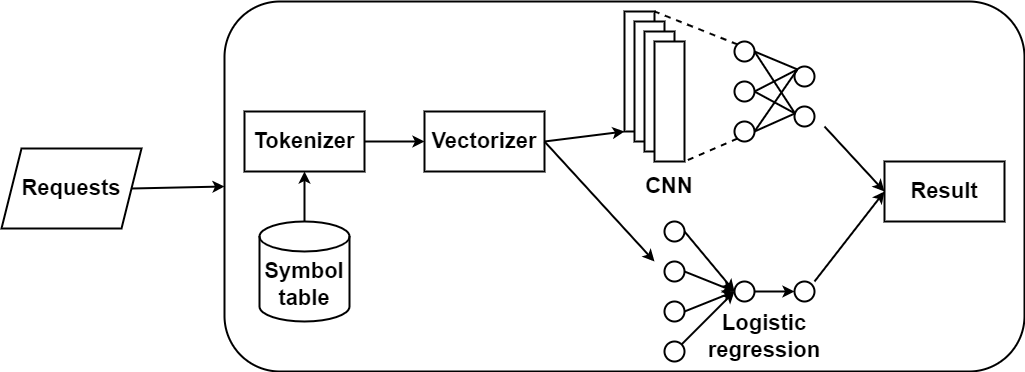
\includegraphics[width=\linewidth, height=10cm,keepaspectratio]{figures/Untitled Diagram.drawio (1).png}
  \caption{The framework of module}
\end{figure}   

\subsection{Logistic regression model}
\hspace{0.5cm}In the prediction process, we train a logistic regression\index{Logistic regression} model to determine whether an incoming request is malicious or not.
\subsubsection{Data Processing}
\hspace{0.5cm}The data acquired, however, wasn't always in the format required for this project, i.e. just the input string. For instance, some of the data were in HTTP, GET, and POST queries. The data was converted into a format appropriate for this purpose to a CSV\footnote{A comma-separated values (CSV) file is a delimited text file that uses a comma to separate values. Each line of the file is a data record.} file using Python scripts.

\subsubsection{Feature engineering}
\hspace{0.5cm}The first part is tokenizing the data. Since our input do not only contain only words and punctuation like normal sentences, we must have an efficient way to tokenize our data (Figure 5.2).

\begin{figure}[!h]
	\centering
	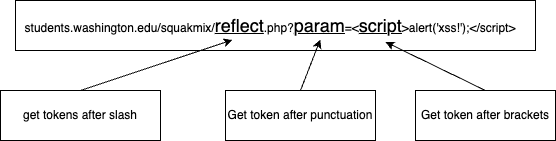
\includegraphics[width=\linewidth, height=10cm,keepaspectratio]{figures/implement1.png}
  \caption{The method of tokenizing data}
\end{figure} 

\newpage
We also eliminate redundant tokens and remove frequently appearing words that are not relevant to the detection process of malicious requests, such as ``localhost'', ``.com'', etc.

Learning algorithms work with numerical features, so we need to convert words into numerical vectors. How does it work? The first entry technique mentioned is called ``Bag-of-words.''\footnote{Bag-of-words is a Natural Language Processing technique of text modelling.}\index{Bag-of-words}
A competent classifier in bag-of-words recognizes patterns in word distribution, which words appear, and how many times for each type of text. However, counting words is not always the best idea. As previously established, a request URL might be exceedingly long, adding bias to our predictions. We used TF-IDF\index{TF-IDF} scores instead of the ``Bag-of-words'' classification since there are words in URLs that are more important than other words e.g. `DROP', `script', `param' etc. Then apply logistic regression\index{Logistic regression}.

\section{CNN classifier}
\label{sec:cnn_classfier}

\subsection{Framework}
\hspace{0.5cm}The framework of classifier is presented in Figure 5.3.
\begin{figure}[!h]
	\centering
	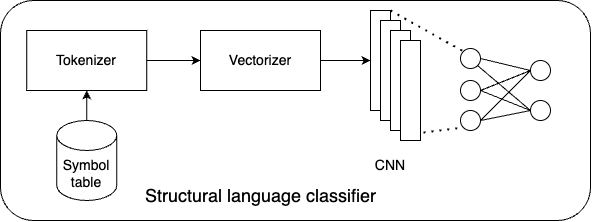
\includegraphics[width=\linewidth, height=10cm,keepaspectratio]{figures/structural.png}
  \caption{Framework of CNN classifier}
\end{figure} 
The request classifier consists of three parts: tokenizer\index{Tokenizer}, vectorizer\index{Vectorizer}, and CNN\index{CNN}. The whole categorizer is built on Python.

The tokenizer\index{Tokenizer} formats the request by utilizing regular expressions to format white spaces and messages and a predetermined set of keywords (symbol table).

The vectorizer vectorizes the request using a small word2vec\index{word2vec} model built by gensim\footnote{Gensim is a Python library for topic modelling, document indexing and similarity retrieval with large corpora. Target audience is the natural language processing (NLP) and information retrieval (IR) community.}. The structured language dataset is used to train the model. The output of the vectorizer\index{Vectorizer} is a list of vectors (with height 150) representing each word of tokens.

The embedded vector is then sent into a trained CNN\index{CNN} to forecast the request's categorization. The architecture is illustrated in Figure 5.4 and detailed as Table 5.1.

\begin{figure}[!h]
	\centering
	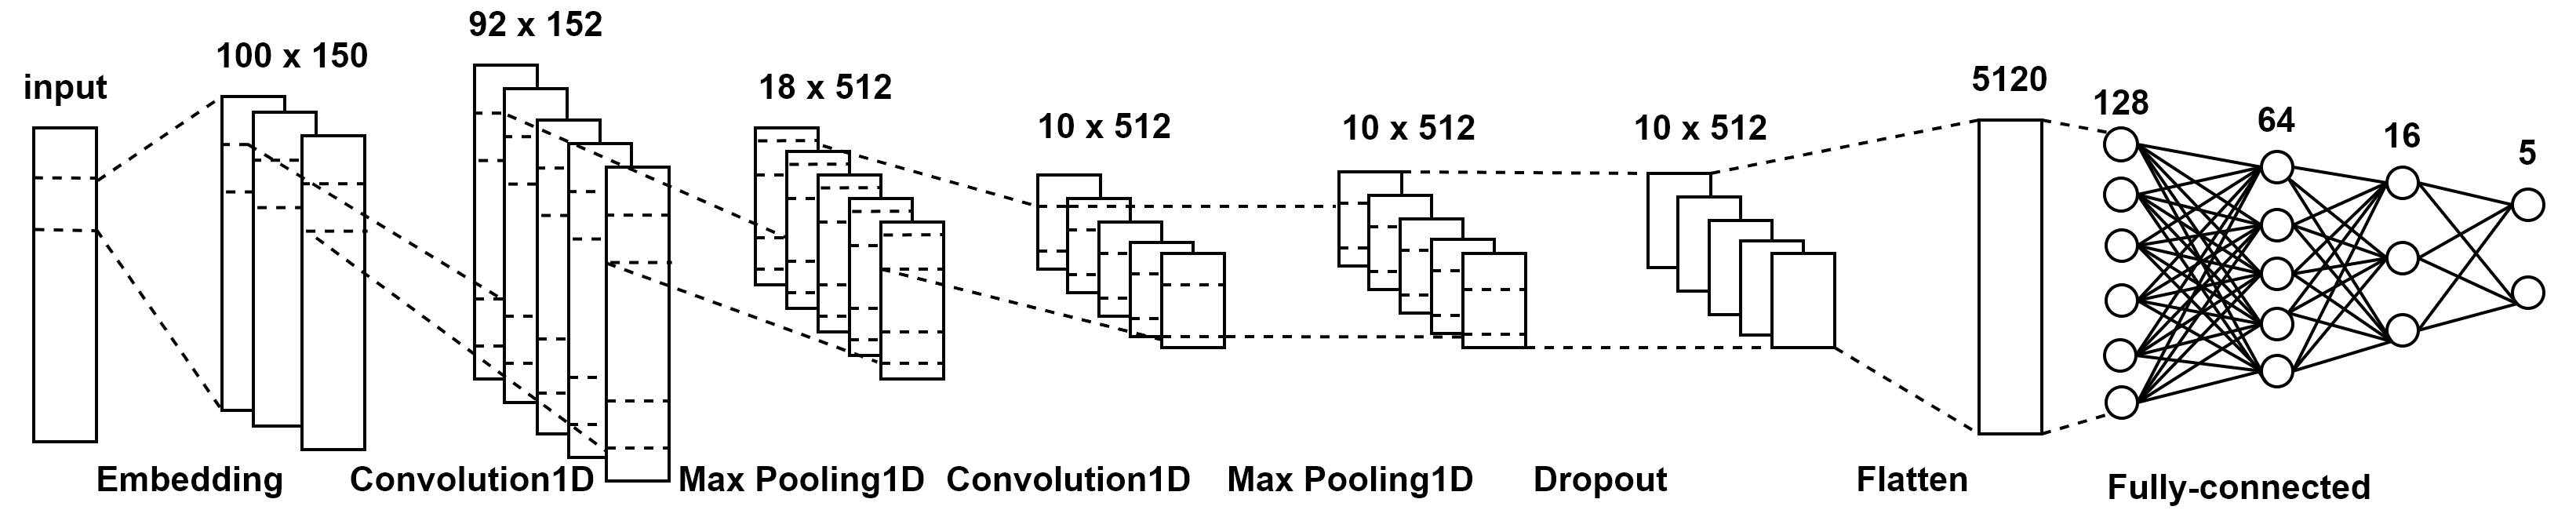
\includegraphics[width=\linewidth, height=10cm,keepaspectratio]{figures/layers.png}
  \caption{Architecture of malicious request validator model.}
\end{figure} 

\begin{table}[!h]
	\begin{tabular}{lrr}
	\hline
	\textbf{Layer (type)}             & \textbf{Output Shape} & \textbf{Amount of parameters} \\ \hline
	embedding (Embedding)             & (None, 100, 150)      & 172447200                     \\
	conv1d (Conv1D)                   & (None, 92, 512)       & 691712                        \\
	max\_pooling1d (MaxPooling1D)     & (None, 18, 512)       & 0                             \\
	conv1d\_1 (Conv1D)                & (None, 10, 512)       & 2359808                       \\
	max\_pooling1d\_1 (MaxPooling1D ) & (None, 10, 512)       & 0                             \\
	dropout (Dropout)                 & (None, 10, 512)       & 0                             \\
	flatten (Flatten)                 & (None, 5120)          & 0                             \\
	dense (Dense)                     & (None, 128)           & 655488                        \\
	dense\_1 (Dense)                  & (None, 64)            & 8256						 \\
	dense\_2 (Dense)                  & (None, 16)            & 1040                         \\ 
	dense\_3 (Dense)                  & (None, 5)             & 85                           
	\\ \hline
	\multicolumn{3}{l}{Total parameters: 176,163,589}                                         \\
	\multicolumn{3}{l}{Trainable parameters: 3,716,389}                                       \\
	\multicolumn{3}{l}{Non-trainable parameters: 172,447,200}                                 \\ \hline
	\end{tabular}
	\caption{\label{demo-table} Architecture specifiations of malicious request validator model.}
\end{table}


The model can be explained as follows.
\begin{itemize}
	\item \textbf{Input data}. The input data of the model is from the word2vec\index{word2vec} model. The data is then embedded using the previous vectorizer with height 150, making the output of the layer a 100 $\times$ 150 neuron matrix. The 3,716,319 parameters of this layer are the embeddings of the word2vec itself, then we have already trained these parameters in the previous vectorizer. This layer is frozen the CNN train starts with the next layer.
	\newpage
	\item \textbf{First 1D CNN layer}. The first layer defines a filter (also called feature detector) of height 9 (also called kernel size). Only defining one filter would allow the neural network to learn one single feature in the first layer. It might not be sufficient, so we will define 512 filters. It allows us to train 512 different features on the first layer of the network. The output of the first neural network layer is a 92 $\times$ 512 neuron matrix. Each column of the output matrix holds the weights of one single filter. With the defined kernel size and considering the length of the input matrix, each filter will contain 92 weights. 
	\item \textbf{First Max pooling layer}. A pooling layer is often used after a CNN layer to reduce the complexity of the output and prevent overfitting of the data. In the thesis, we chose a size of five. It means that the size of the output matrix of this layer is only one-fifth of the input matrix. 
	\item \textbf{Second 1D CNN layer}. Another sequence of 1D CNN\index{CNN} layers follows to learn higher-level features. The output matrix after those two layers is an 18 $\times$ 512 matrix. 
	\item \textbf{Second Max pooling layer}. One more pooling layer to further avoid overfitting. The output matrix has a size of 10 $\times$ 512 neurons. For each feature detector, ten weights remain in the neural network on this layer. 
	\item \textbf{Dropout layer}. The dropout layer\index{Dropout layer} will randomly assign 0 weights to the neurons in the network. Since we chose a rate of 0.3, 30\% of the neurons will receive a zero weight. With this operation, the network becomes less sensitive to react to smaller variations in the data. Therefore it should further increase our accuracy\index{Accuracy} on unseen data. The output of this layer is still a 10 $\times$ 512 matrix of neurons. 
	\item \textbf{Flatten layer}. This layer\index{Flatten layer} will compress the 10 $\times$ 512 matrix from the previous layer into one vector with height 5120, preparing for the classification phase. 
	\item \textbf{Four fully-connected layers}. Four final layers will force the vector of height 5120 to a vector of 5 since we have five classes (plain text, client-side script, server-side script, shell script, and SQL). This reduction is made by matrix multiplications. Since the gap between the two vectors is too large (5120 and 5), we need five layers. The first three layers reduce the height from 5120 to 128, 128 to 64, and 64 to 16 respectively, using ReLU\footnote{
		Rectifier Linear Unit (ReLU) function: $g(z) = max(0, z)$
	} as the activation function. The final layer reduces from size 16 to 5. Softmax\index{Softmax} is used as the activation function. It forces all three outputs of the neural network to sum up to one. The output value will therefore represent the probability for each of the three classes.
\end{itemize}
\newpage
\hspace{0.5cm}The CNN\index{CNN} focuses on identifying typical requests (plain text) to decrease the FP\index{False positive} of rule-based\index{Rule-based} techniques. Then the model is converted to plain text using class weights. The weight for plain text is 5, whereas for others is 1. As a five-label loss function\index{Loss function}, the training method employs Mean squared error\footnote{
	Mean Squared Error function: $MSE = \frac{1}{n}\sum_{i=1}^{n}(Y_i-\widehat{Y}_i)^2$
} loss function. Because others are programming languages, their predicted distributions are similar. When the loss function is Sparse Categorical Cross-Entropy\hspace{-0.15cm}
\footnote{
	Sparse categorical cross-entropy loss function: $-\sum_{c=1}^My_{o,c}\log(p_{o,c})$
}, which has a harsh punishment for classification errors, the model may constantly alternate the prediction of these two labels. Adam\index{Adam (algorithm)} is used as the model optimizer with learning rate\index{Learning rate} of 0.005, $\beta_1$ = 0.9, $\beta_2$ = 0.999, and $\varepsilon$ = 1. We are focused on the accuracy\index{Accuracy} of the model.

